\subsubsection{}
\label{sec:development:arch:pp:vapor}

\textbf{Vapor} -- веб фреймворк для языка Swift, предоставляющий выразительный и простой в использовании набор модулей для разработки веб-сайтов, \gls{api} и облачных решений\cite{vapor:github}.

\textit{Vapor} является одним из трёх самых популярных веб-фреймворком для разработки приложений на языке свифт, имеет самую большую пользовательскую базу, поддержку со стороны компании Apple, высокие показатели в тестах производительности и стабильности. Начиная с третьей версии, фреймворк использует принципы неблокирующего ввода-вывода, а конкретно имплементацию компании Apple, \textit{SwiftNIO}, которая рассмотрена в пункте \ref{sec:development:arch:pp:nio}.

\textit{Vapor} предоставляет богатый набор модулей, значительно упрощающих разработку:

\begin{itemize}
	\item авторизация;
	\item криптография;
	\item сессии;
	\item работу с локальным хранилищем;
	\item имплментацию паттерна Future/Promise;
	\item имплементацию протокола \gls{http} и поддержку \gls{http} 2;
	\item адаптеры ко многим популярным базам данных;
	\item \gls{api} для работы с хранилищем Redis.
	\item собственную \gls{orm};
	\item язык и инструмент рендеринга шаблонов HTML;
	\item работа с файловой системой и общее взаимодействие с операционной системой;
	\item имплементацию динамических \gls{di} контейнеров;
	\item имплементацию \gls{ws}.
\end{itemize}

Как и остальные современные веб-фреймворки, \textit{Vapor} работает по следующему принципу\cite{server-side-swift}:
\begin{itemize}
	\item разработчик описывает \textit{роутинг} в своём приложении;
	\item разработчик описывает \textit{модели базы данных};
	\item за каждым возможным путём закрепляется собственный \textit{обработчик}, семейства обработчиков объединяются в \textit{контроллеры};
	\item логика сервера описывается в обработчиках, в случае с Vapor, в обработчик передаётся контейнер, позволяющий получить параметры запроса и асинхронно сформировать ответ;
	\item разработчик описывает общую конфигурацию приложения и регистрирует сервисы.
\end{itemize}


На рисунках \ref{sec:development:arch:pp:vapor:code:route} и \ref{sec:development:arch:pp:vapor:code:db} приведены примеры регистрации нового обработчика и описания модели базы данных соответственно.

\begin{figure}[h]
  \centering
    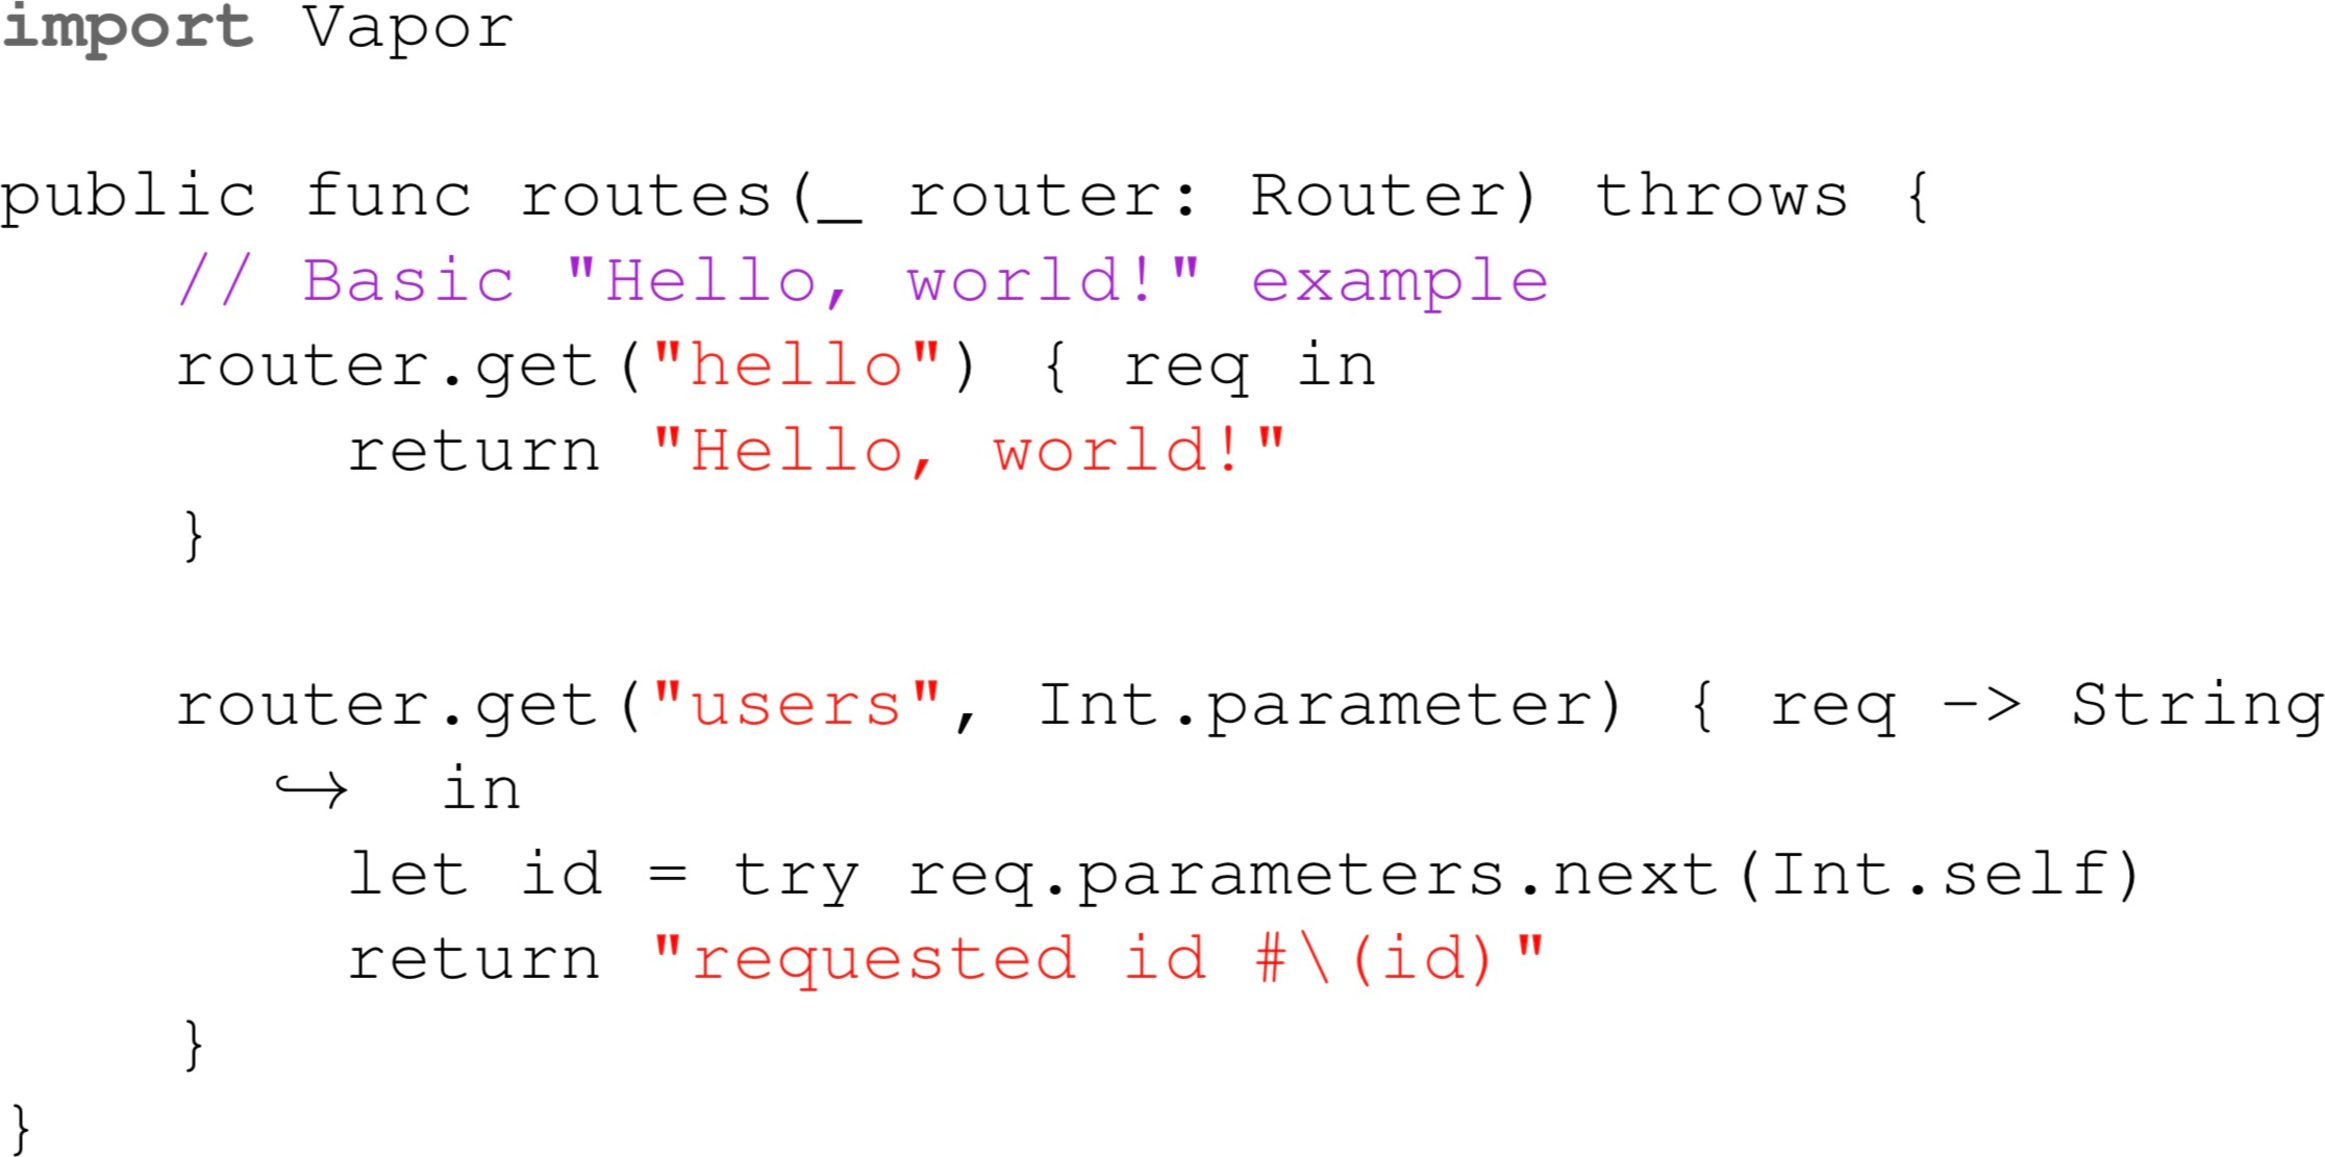
\includegraphics{inc/img/listing/vapor_route}
  \caption{Пример описания пути и обработчика в Vapor}
  \label{sec:development:arch:pp:vapor:code:route}
\end{figure}

\begin{code}
	\lstinputlisting{inc/src/vapor_route.swift}
   \caption{Пример описания пути и обработчика в Vapor}
   \label{sec:development:arch:pp:vapor:code:route}
\end{code}

\begin{code}
	\lstinputlisting{inc/src/vapor_db.swift}
   \caption{Пример модели базы данных в Vapor}
   \label{sec:development:arch:pp:vapor:code:db}
\end{code}

Фреймворк выбран в качестве основы для разработки серверной части \gls{pp} исходя из популярности, частоты и качества обновлений, поддержки со стороны Apple и набора готовых модулей, полностью покрывающих требования к серверной части настоящего программного продукта.